%----------------------------------------------------------------------------------------
%	Technical Overview
%----------------------------------------------------------------------------------------

\chapter{Technical Overview}

The smart scale containes many different parts that work together to create a full system, as seen in figure \ref{fig:sys_diagram}. 

\begin{figure}[!ht]
    \centering
    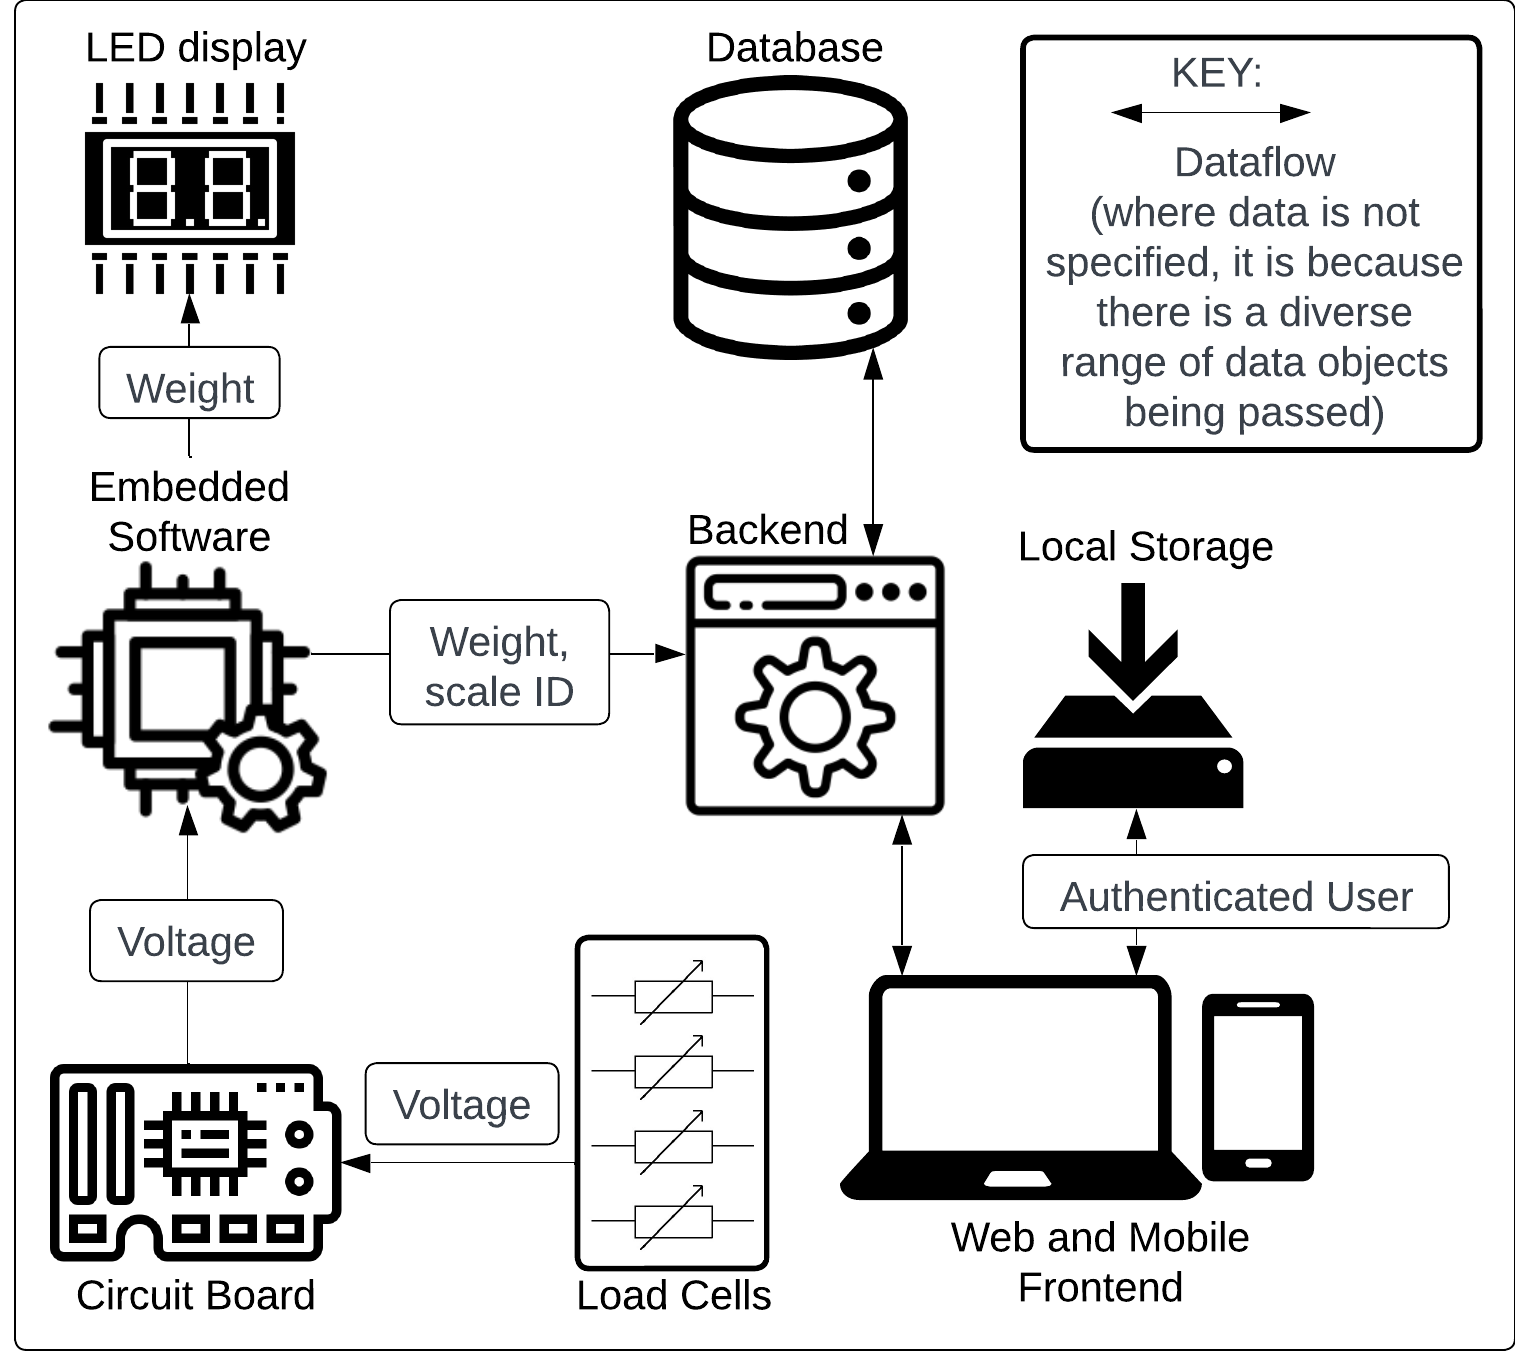
\includegraphics[scale=0.9]{hardware_overview.png}
    \caption{System diagram}
    \label{fig:sys_diagram}
\end{figure}

The scale has load cells which measure the weight as a voltage, and this voltage is then amplified and processed before being sent to the Analog to Digital Converter (ADC) of the scale's microcontroller. This embedded component averages thousands of samples to reach an accurate weight, ensuring that the SPCA staff have a clear measure of the dog's weight. There is a 7-segment display that shows this weight, and flashes when the weight has stabilised. At this point, the embedded component sends an http request to the software backend. This LED display allows the user more confidence in the measurement as they have more insight into the process, and means that the scale can be used even if the WiFi or software is not working. 

The software backend includes a database and an application programming interface (API) that allows other parts of the software to interact with the database. An SQLite database is used for its high performance and efficiency, and its compatibility with a range of popular languages. The software includes two frontend components: a web platform, and a mobile platform. This will allow the user to interact with the data stored in the backend, and perform many actions such as saving a dog's weight, viewing statistics, and chatting with other staff members. The platforms are coded in popular languages that will ensure more features can be implemented in the future. The applications are user-friendly and easy to learn, so the SPCA will not have to devote a large amount of time to training their staff with the technology. The hardware and software work together to ensure that the SPCA can easily weigh and manage the dogs in their care. 
